\documentclass{beamer}

\usepackage{amsfonts}
\usepackage{amsmath}
\usepackage{longtable}
\usepackage{csquotes}
\usepackage{standalone}

\usepackage{graphicx}
\graphicspath{{../pictures/}}

\usepackage{tikz}
\usetikzlibrary{shapes, calc, arrows, decorations.markings,
  decorations.pathmorphing, decorations, patterns, chains, snakes,
  backgrounds, positioning, fit, petri}
\newcommand{\inputpicture}[1]{\input{../drawings/#1}}

\usepackage{listings}
\lstset{language=C, basicstyle=\ttfamily, breaklines=true, keepspaces=true,
  keywordstyle=\color{blue}}

\usepackage{bytefield}

\usefonttheme{professionalfonts}
\usefonttheme{serif}
\usepackage{fontspec}
\setromanfont{CMU Serif}
\setsansfont{CMU Sans Serif}
\setmonofont{CMU Typewriter Text}

\usepackage{hyperref}
\hypersetup{colorlinks=true, linkcolor=black, filecolor=black, citecolor=black,
  urlcolor=blue , pdfauthor=Evgenii Iuliugin <yulyugin@gmail.com>,
  pdftitle=Fundamentals of Full-Platform Simulation}

\usepackage{underscore}
\usepackage{amsthm}

\subtitle{Fundamentals of Full-Platform Simulation}
\subject{Lecture}
\date{\today}

\author[Evgenii Iuliugin]{
  Evgenii Iuliugin \small{\href{mailto:yulyugin@gmail.com}{yulyugin@gmail.com}}}
\typeout{Copyright 2021 Evgenii Iuliugin}

\usetheme{Berlin}
\setbeamertemplate{navigation symbols}{}

\newcommand{\finalslide}{
    {\huge{Thank you!}\par}

    \vfill
    Slides and material are available at
    \url{https://github.com/yulyugin/sim-lectures}
    \vfill

    \tiny{\textit{Note}: All trademarks are the property of their respective
        owners.
        The presented point of view reflects the personal opinion of the author.

        %All the materials are licensed under the Creative Commons
        %Attribution-NonCommercial-ShareAlike 4.0 Worldwide. To view a copy of
        %this license, visit
        %\url{http://creativecommons.org/licenses/by-nc-sa/4.0/}.
    }
}

\title{Потактовая симуляция}

\begin{document}

\begin{frame}
    \maketitle
\end{frame}

\begin{frame}
    \tableofcontents
\end{frame}

\begin{frame}{На прошлой лекции}
\begin{itemize}
    \item Модель, управляемая исполнением (функциональная модель)
    \item Модель, управляемая событиями (DES)\pause
    \item \textbf{Модель, моделирующая каждый такт} (time-stepped)
\end{itemize}
\end{frame}

\begin{frame}{Questions}
\begin{itemize}
\item Сколько бит в машинном слове? \pause
\item Что лучше — MMIO или PIO?\pause
\item Может ли архитектура быть и не little, и не big-endian?
\end{itemize}
\end{frame}

\section{Потактовая модель}

\begin{frame}{Что моделируем}
\centering

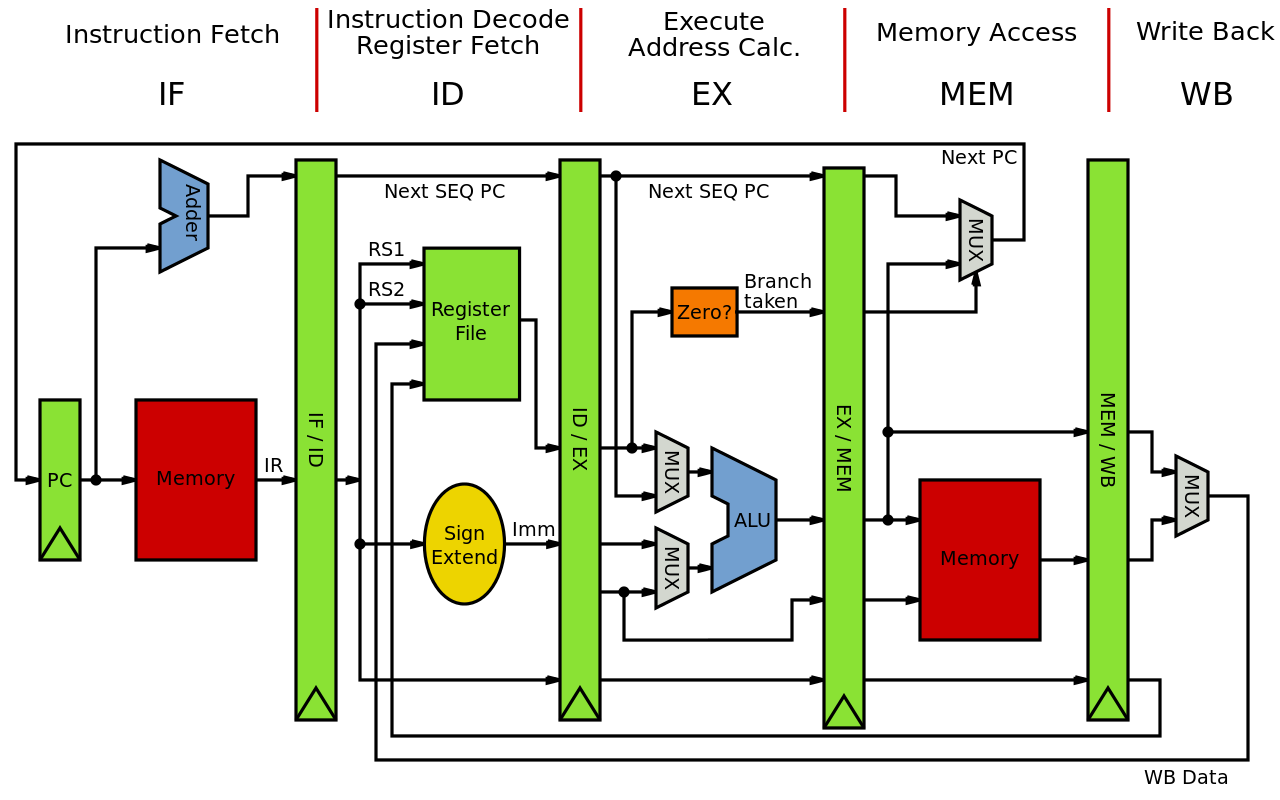
\includegraphics[width=\textwidth]{./mips-arch}

\tiny{\url{http://commons.wikimedia.org/wiki/File:MIPS_Architecture_(Pipelined).svg}}
\end{frame}

\begin{frame}{Проблемы}
\begin{itemize}
    \item Функциональная модель — не работает (слишком грубая)
    \item DES — применима, но неудобная абстракция
\end{itemize}

\inputpicture{des-long}

\end{frame}

\begin{frame}{Особенности}

\inputpicture{features}
\end{frame}

\begin{frame}{Проблемы}
\begin{itemize}
\item Длительность одной операции у разных узлов могут быть различными
\item Как проверять готовность «медленных» узлов?
\item Результаты обработки данных должны появляться не ранее, чем на такте, следующим за текущим
% \item Нельзя в произвольном порядке обновлять состояние блоков
\end{itemize}

\end{frame}

\section{Функции и порты}

\begin{frame}{Решение}
Отделим:
    \begin{itemize}
    \item Функции узлов
    \item Время, затрачиваемое на их выполнение
    \item Внутреннее состояние узлов
    \end{itemize}
\end{frame}

\begin{frame}{Функциональный элемент}
Результат готов «мгновенно» при наличии входных данных

\vfill
\centering
\inputpicture{pure-function}

\end{frame}

\begin{frame}{Порт}
Очередь фиксированной задержки

Ширина $N$ бит, задержка 1 такт

\vfill
\centering
\inputpicture{delay-line}

\end{frame}

\begin{frame}{Правило соединения}

\begin{itemize}
\item Функции не могут соединяться непосредственно друг с другом
\item Чередующиеся фазы симуляции:
\begin{enumerate}
    \item симуляция функций;
    \item симуляция передачи результатов
\end{enumerate}
\end{itemize}
\end{frame}

\begin{frame}{Модель с портами: фаза 1}

\centering
\inputpicture{cycle-phase1}

\end{frame}

\begin{frame}{Модель с портами: фаза 2}

\centering
\inputpicture{cycle-phase2}

\end{frame}


\section{Детали реализации}

\begin{frame}{Готовность данных}

\centering
\inputpicture{valid}

\end{frame}

\begin{frame}{Могут ли функциональные элементы иметь память?}

\centering
\inputpicture{state-storing}

\end{frame}

\begin{frame}{Композиция узлов}

\centering
\inputpicture{ports-compose}

\end{frame}

\begin{frame}{Связь функциональной и потактовой моделей}

\centering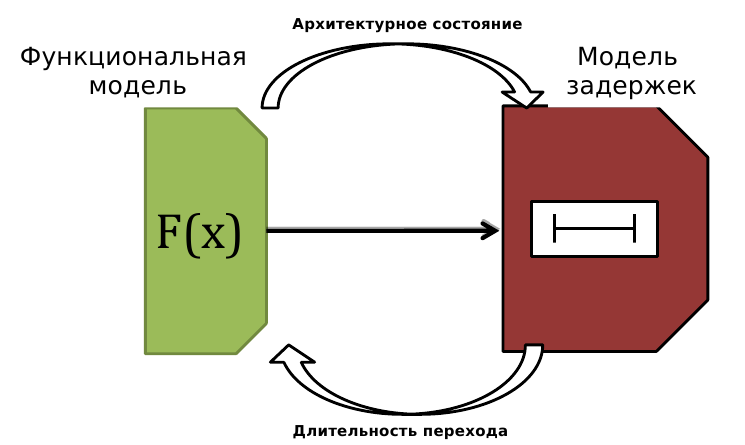
\includegraphics[width=0.8\textwidth]{functional-cycle-precise-connection}

\end{frame}

% \begin{frame}{Диаграмма моделируемой системы}
% 
% \end{frame}


\begin{frame}[allowframebreaks]{Литература}
\begin{thebibliography}{99}
    \bibitem{patterson-hennessy} Дэвид Паттерсон и Джон Хэннесси. Архитектура компьютера и проектирование компьютерных
систем. 4-е изд. Питер, 2012.

\bibitem{Asim} Joel Emer, Pritpal Ahuja, Eric Borch, Artur Klauser, Chi-Keung Luk, Srilatha Manne, Shubhendu S. Mukherjee,
Harish Patil, Steven Wallace, Nathan Binkert, Roger Espasa, Toni Juan. Asim: A Performance Model Framework // Computer 35 (2002), p. 68–76.

\bibitem{baida} Ю.В. Байда. Методы разработки и тестирования аппаратных потактовых моделей микропроцессоров на программируемых логических интегральных схемах. Дисс. к.т.н. — 2013
\end{thebibliography}
\end{frame}

\begin{frame}{На следующей лекции}
\centering

Параллельная симуляция, управляемая исполнением (MPonMP)

\end{frame}


\begin{frame}

{\huge{Спасибо за внимание!}\par}

\vfill

Слайды и материалы курса доступны по адресу \url{http://is.gd/ivuboc} % http://atakua.doesntexist.org/wordpress/simulation-course-russian/

\vfill

\tiny{\textit{Замечание}: все торговые марки и логотипы, использованные в данном материале, являются собственностью их владельцев. Представленная здесь точка зрения отражает личное мнение автора, не выступающего от лица какой-либо организации.}

\end{frame}

\end{document}
